\documentclass[nohyperref]{article}

% Recommended, but optional, packages for figures and better typesetting:
\usepackage{microtype}
\usepackage{graphicx}
\usepackage{subfigure}
\usepackage{booktabs} % for professional tables

% hyperref makes hyperlinks in the resulting PDF.
% If your build breaks (sometimes temporarily if a hyperlink spans a page)
% please comment out the following usepackage line and replace
% \usepackage{icml2022} with \usepackage[nohyperref]{icml2022} above.
\usepackage{hyperref}


% Attempt to make hyperref and algorithmic work together better:
\newcommand{\theHalgorithm}{\arabic{algorithm}}

% Use the following line for the initial blind version submitted for review:
%\usepackage{icml2022}

% If accepted, instead use the following line for the camera-ready submission:
 \usepackage[accepted]{icml2022}

% For theorems and such
\usepackage{amsmath}
\usepackage{amssymb}
\usepackage{mathtools}
\usepackage{amsthm}

% if you use cleveref..https://www.overleaf.com/project/64edfc2e136251c90ff7c481
\usepackage[capitalize,noabbrev]{cleveref}

%%%%%%%%%%%%%%%%%%%%%%%%%%%%%%%%
% THEOREMS
%%%%%%%%%%%%%%%%%%%%%%%%%%%%%%%%
\theoremstyle{plain}
\newtheorem{theorem}{Theorem}[section]
\newtheorem{proposition}[theorem]{Proposition}
\newtheorem{lemma}[theorem]{Lemma}
\newtheorem{corollary}[theorem]{Corollary}
\theoremstyle{definition}
\newtheorem{definition}[theorem]{Definition}
\newtheorem{assumption}[theorem]{Assumption}
\theoremstyle{remark}
\newtheorem{remark}[theorem]{Remark}

% Todonotes is useful during development; simply uncomment the next line
%    and comment out the line below the next line to turn off comments
%\usepackage[disable,textsize=tiny]{todonotes}
\usepackage[textsize=tiny]{todonotes}


% The \icmltitle you define below is probably too long as a header.
% Therefore, a short form for the running title is supplied here:
\icmltitlerunning{Urban Shade Finder}

\begin{document}

\twocolumn[
\icmltitle{Urban Shade Finder \\
           Machine Learning Workshop 2023}

\icmlsetsymbol{equal}{*}

\begin{icmlauthorlist}
\icmlauthor{Tomer Klajman}{equal,tau}
\icmlauthor{Uri Alon}{equal,tau}
\icmlauthor{Adi Sharfaizen}{equal,tau}
\icmlauthor{Matan Abudy}{equal,tau}
\end{icmlauthorlist}

\icmlaffiliation{tau}{Department of Computer Science, Tel-Aviv University, Israel}

\vskip 0.3in
]

% this must go after the closing bracket ] following \twocolumn[ ...

% This command actually creates the footnote in the first column
% listing the affiliations and the copyright notice.
% The command takes one argument, which is text to display at the start of the footnote.
% The \icmlEqualContribution command is standard text for equal contribution.
% Remove it (just {}) if you do not need this facility.

%\printAffiliationsAndNotice{}  % leave blank if no need to mention equal contribution
\printAffiliationsAndNotice{\icmlEqualContribution} % otherwise use the standard text.

\begin{abstract}
This paper presents a digital tool for urban shade optimization using street-level imagery data and machine learning models. Given the increasing temperatures and associated health risks in many city environments, this study provides a valuable tool for smart urban planning and efficient resource allocation. This project used Google Street View data and a streamlined pipeline for transforming panoramic images into a hemispheric view, segmenting and classifying objects within the image, and integrating a sun trajectory model. The digital tool demonstrated robust performance in real-world scenarios, achieving an accuracy of 81\% in comparison with ground truth data. Furthermore, the accuracy of a derived model for predicting sun and shade patterns on either side of a sidewalk reached up to 92\%. These findings indicate a promising application of this tool in promoting urban well-being through enhanced shade provision.
\end{abstract}

\section{Introduction}
\label{introduction}
This project was born out of the increasing need for shade in urban environments. High temperatures during summer months in many cities pose a major issue for the well-being of pedestrians,  an issue that will only become more prevalent with global warming. Unfortunately, there are currently no good and precise tools to assess where in a city there is shade and where it is sunny. As a result, cities lack the necessary information to invest their resources efficiently into improving the shade situation.

To address this issue, the project aims to develop a digital tool for shade optimization. This tool will enable the planning of solutions for shade provision at the street level, ultimately improving the well-being of the city's residents. We achieve this using street-level imagery data and machine learning models that helps us assessing the shade situation on the street.

\section{The Data}
\label{data}
To achieve our goal of democratizing urban shade solutions, we have chosen to use Google Street View (GSV) data to create our assessments. Since GSV is free to use and available for many cities around the world, we aimed to create a model that is useful and accessible for public and private use.

Using GSV, we were able to retrieve panoramic images of specific coordinates by using an undocumented API that provides a list of panoramas in close proximity to a given coordinate. If a panoramic image is unavailable for specific coordinates, we select the closest available image. In some cases, we may not have access to the most up-to-date images from GSV, so we make our best effort to select the most recent picture available.

\begin{figure}[ht]
\begin{center}
\centerline{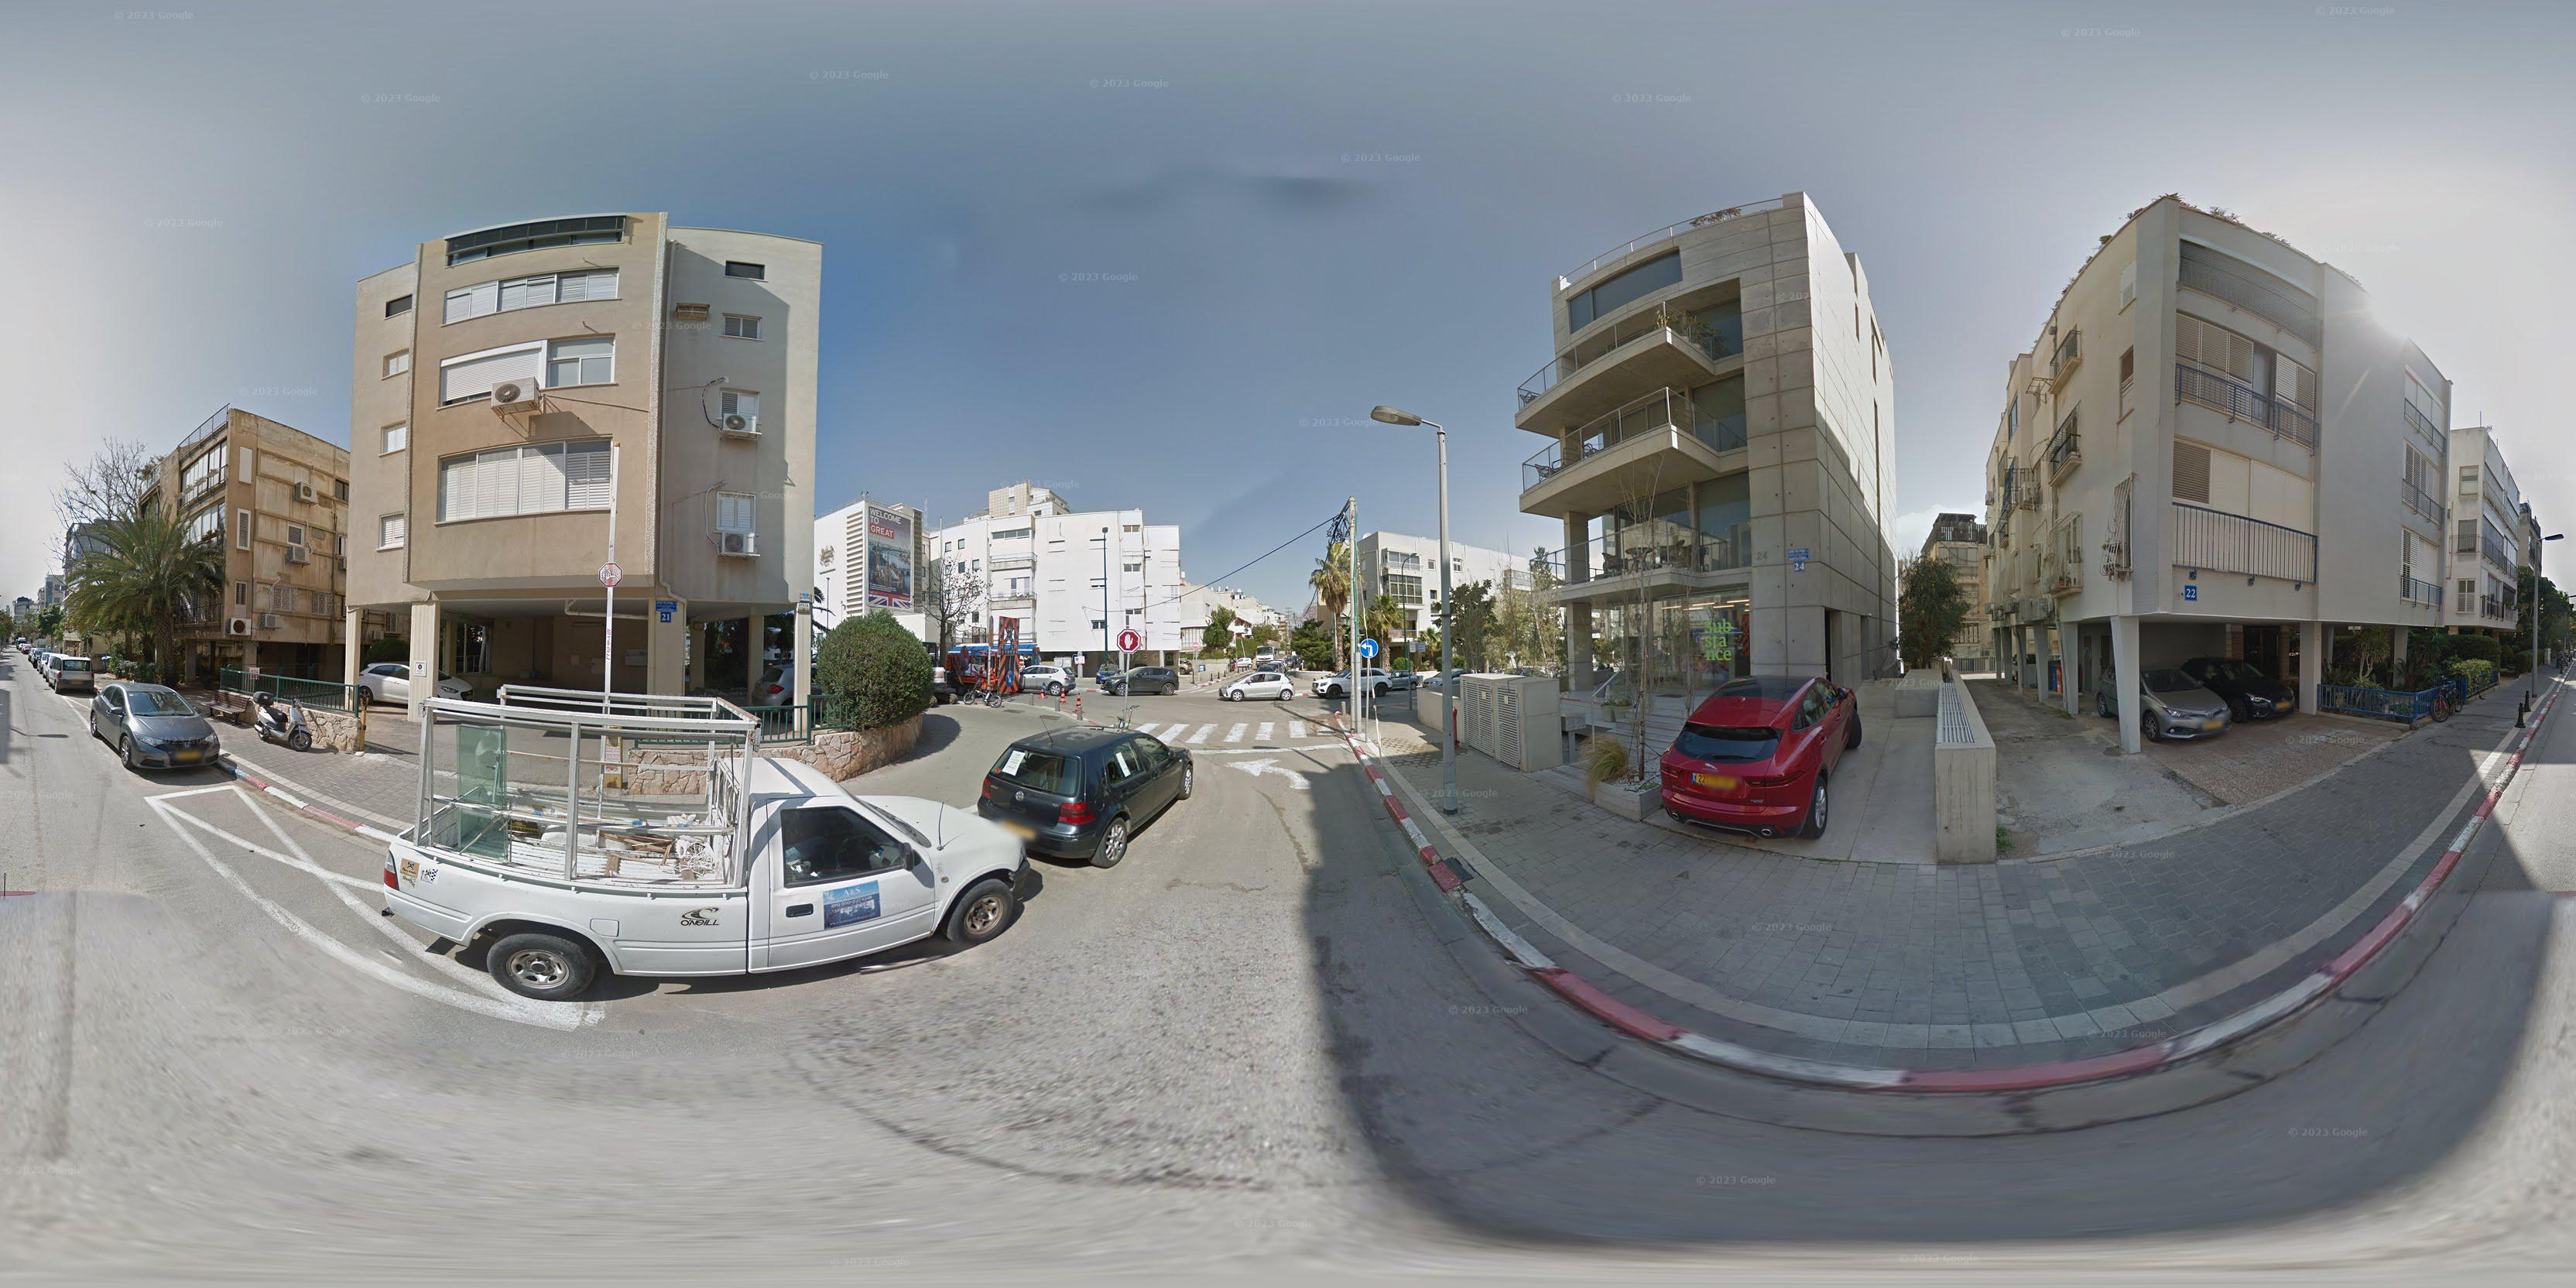
\includegraphics[width=\columnwidth]{example_panorama.jpg}}
\caption{Panoramic image of latitude 32.08736640506768, longditude 34.77184320109989}
\vskip -0.2in
\end{center}
\end{figure}

However, this step posed various challenges, despite its seeming straightforwardness. The first challenge was the use of the undocumented API. Previous works on estimating solar radiance or shade using street view images almost exclusively used this undocumented API, as it was easier to retrieve panoramic images than the official API (\citet{rs14020260}, \citet{GONG2019547}, \citet{LI2018109}). We wanted to continue in the same direction and use the same API to retrieve panoramic images, but this presented two main issues. Firstly, almost no previous work had released an open-source version of the code. Secondly, even if we could find open-source code, it was mostly obsolete as the API has changed significantly.

To solve these issues, we partnered with a new open-source GSV Python package called \texttt{streetview} (\url{https://github.com/robolyst/streetview}). We first used it as an initial proof-of-concept, and then contributed to it some of our own code to support more use cases we encountered during our research.

\section{Methods}
\label{methods}
To comprehensively assess urban shade, we aim to estimate the Sky View Factor (SVF). SVF is a numerical quantity that indicates the proportion of visible sky from a certain point. It measures the "openness" or visual obstruction in an urban setting. By estimating SVF and integrating it with a sun trajectory model, we can determine when sun radiance passes through "open" sky and when it is blocked by buildings or trees. To achieve this, we have established a streamlined pipeline consisting of the following steps:

\begin{enumerate}
    \item \textbf{Transformation}: Acquire and adapt panoramic images into a hemispheric view, readying them for detailed analysis.
    
    \item \textbf{Segmentation}: Identify and isolate all distinct objects within the transformed image.
    
    \item \textbf{Classification}: Categorize the segmented objects into specific labels to determine their nature and role in shade creation.
    
    \item \textbf{Sun Model Integration}: Overlay a sun trajectory model onto the classified image to ascertain areas exposed to direct sunlight.
\end{enumerate}

The subsequent sections delve deeper into the specifics of each step.

\begin{figure}[ht]
\begin{center}
\centerline{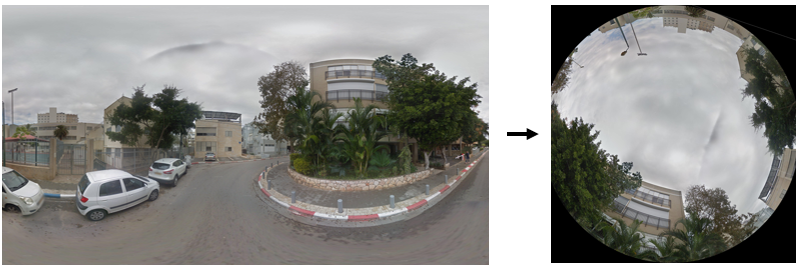
\includegraphics[width=\columnwidth]{pipeline-1.png}}
\caption{Converting panoramic image to hemispheric image}
\end{center}
\vskip -0.2in
\end{figure}

\begin{figure}[ht]
\begin{center}
\centerline{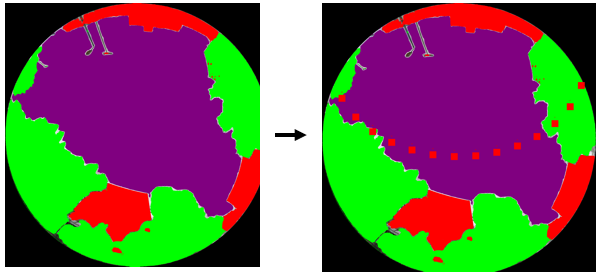
\includegraphics[width=\columnwidth]{pipeline-2.png}}
\caption{Classification, segmentation and sun model integration}
\end{center}
\vskip -0.2in
\end{figure}

\subsection{Turning Panoramas to Hemispheric Image}
After obtaining the panorama image, we needed to convert it to a hemispheric image. This involved first converting the panorama into a fisheye view, and then rotating it to align with a real coordinate system and compass rose. This transformation allowed us to segment and classify elements in the panorama that may block the sun and create shade in specific coordinates.

To make the fisheye transformation, we relied on code from \citet{li2019pedestrian} which in its turn was adapted from the MIT Senseable City Lab based on \citet{rs9050411}.

To make the rotation, we retrieved the yaw angle from the undocumented GSV API. The yaw angle refers to the rotation around the vertical axis of a vehicle, altering the horizontal alignment of a photo capture device like the 360-degree camera utilized in the Google Street View vehicle. Using the yaw angle, we were able to rotate the hemispheric image so that it aligns with the compass rose, with north always pointing upwards.

\subsection{Segmentation}
To segment objects in our hemispheric images, we deployed Meta's "Segment Anything Model" (SAM). SAM stands out for its capacity to autonomously identify and segment all objects present in an image without the need for specific prompts, such as clicks or bounding boxes. Trained on the vast SA-1B dataset containing over 1 billion masks, SAM's proficiency in generalization ensures precise segmentation even in complex urban scenarios. SAM worked well out of the box, and after a few iterations of tuning it's hyper-parameters we were able to leverage its unique ability to automatically find and mask all objects in a given image for our task.

\subsection{Classification}
Post-segmentation, each segmented mask from the hemispheric images was subjected to classification to categorize it into one of the following labels: "building", "sky", "tree" or other. For this task, we employed the SegFormer model. SegFormer is an advanced semantic segmentation framework which unifies Transformers with lightweight multilayer perception (MLP) decoders. Our chosen version of SegFormer was trained by Nvidia on the ADE20K dataset. This dataset, with over 20K scene-centric images, provides comprehensive annotations at the pixel level, covering 150 semantic categories. These range from general elements like sky and road to specific objects like cars and people, making it a fitting foundation for our classification requirements in assessing urban shade. The model predicted on each mask it's most probable label, where each pixel in the mask was colored in a distinct color matching its corresponding label, as detailed above, and that modified image was returned to be used in the sun model.

\subsection{Sun Model}
Upon acquiring a segmented fish-eye image of the sky, we integrated a dynamic sun model onto the image. This integration allows us to determine the periods during which our specified location is exposed to direct sunlight.

Given the precise coordinates and a specific date, we can calculate the sun's trajectory throughout the day. By analyzing the segmentation of the pixels corresponding to the sun's position, we can effectively determine if our location is in the sun or shade.

The primary steps for this analysis are:

\begin{enumerate}
    \item \textbf{Convert the segmented fisheye image into a \texttt{numpy} array.}
    By converting the image into a \texttt{numpy} array, we create a structured format that facilitates further processing and analysis within our computational environment.

    \item \textbf{Calculate the sun's position based on date, time, and location.}
    This calculation is achieved using the \texttt{sunfinder} Python package, which provides accurate sun positioning data based on geographical inputs and timestamps.

    \item \textbf{Overlay the sun's position on the fisheye image.}
    To do this, we convert the sun's azimuth and elevation angles to x and y coordinates suitable for our fisheye image by using trigonometric operations.
    
    \item \textbf{Determine the shade or sunlight status by assessing the sun's position against the segmented pixels of the image.} Since the image was already segmented, the logic was simple - sunlight if the pixel was classified as sky, and shade otherwise.
\end{enumerate}

\section{Sidewalk Shifting}
\label{sidewalk-shifting-method}
Initially, our objective was to enhance the model's accuracy by shifting the "point-of-view" of the image from the middle of the road to the sidewalks. This shift could allow us to use the pavements as the reference point, thereby providing more precise and pertinent information for pedestrians.

To achieve this, we explored the possibility of employing NeRF (Neural Radiance Fields) for conducting this shift. However, subsequent investigation and consultation with field experts such as Dr. Amit Bermano led us to the conclusion that this solution is not suitable for our specific problem.

Consequently, we opted to approach this issue from a different perspective. Our aim was to develop a model capable of, given a set of coordinates, the heights of the buildings on both sides of the street, and the width of the street, determining whether there is shade or sunlight on each side of the sidewalks.

The core of our solution leans heavily on trigonometry. At a fundamental level, the shade of a building on the opposite side of a street can be determined by the sun's elevation angle and the height of the building. The key relationship used is the tangent function, which relates the angle of elevation of the sun to the height of the building and the distance of the shadow it casts:
\[
\tan(\theta) = \frac{h}{b}
\]
Where:
\begin{itemize}
    \item \(\theta\) is the sun's elevation angle,
    \item \(h\) is the height of the building, and
    \item \(b\) is the distance from the base of the building to the end of the shadow.
\end{itemize}

Given this relationship, by knowing \(\theta\) and \(h\), we can solve for \(b\), the distance of the shadow on the ground. Depending on the sun's azimuth (its direction in the horizontal plane), the shadow can be cast from the building on the left or the right. 

Furthermore, by introducing the concept of the street's direction (or orientation), we can further refine which building will cast a shadow and where the shadow will land on the street. This orientation, combined with the azimuth, allows us to calculate an effective shadow distance \(b'\), which is the shadow's projection on the street:
\[
b' = b \times \cos(\delta)
\]
Where:
\begin{itemize}
    \item \(b\) is the original shadow distance, and
    \item \(\delta\) is the difference between the sun's azimuth and the street's direction.
\end{itemize}

By iterating this model over various times of the day, we can deduce at which hours the pavements, and by extension, the whole street, are in shade or sunlight.

\section{Results}
\label{results}
\subsection{GSV to Sun Model}

To validate the performance of our urban shade assessment tool, we performed an evaluation using a dataset provided to us by our colleagues at Tel Aviv University's Faculty of Architecture. This dataset contained 21  locations within Tel Aviv, each annotated with sun or shade statuses across five separate time slots across a day. This resulted in a total of 105 labeled data points which we considered the ground truth.

Upon comparing our solution's outputs against this ground truth dataset, we achieved an accuracy of 81\%. Such results emphasize the potential and robustness of our solution, which does not require manual measurements, in real-world scenarios.


\subsection{Sidewalk-Shifting}
\label{sidewalk-shifting-results}
In order to validate our sidewalk-shifting prediction model, we conducted a randomized selection of a specific point within Tel Aviv. At this chosen location, we possessed detailed records of sun and shade patterns throughout the day on both sides of the sidewalks. The building heights were obtained from publicly available data provided by the Tel Aviv Municipality's Geographic Information System (GIS) portal (\url{gisn.tel-aviv.gov.il})

Our analysis yielded an accuracy rate of 92\%. Notably, we achieved perfect accuracy for most predictions, with only one exception: there was a single instance where our model mispredicted shade on the left sidewalk.

For a visual representation, the shading and sunlit areas are denoted by blue and yellow colors respectively on the provided diagrams (see Appendix \ref{sidewalk-predictions}), showing the shade prediction at the point throughout the day. For convenience, we have attached a sample predictions for 8AM in Figure \ref{prediction8}.

\begin{figure}[ht]
\vskip 0.2in
\begin{center}
\centerline{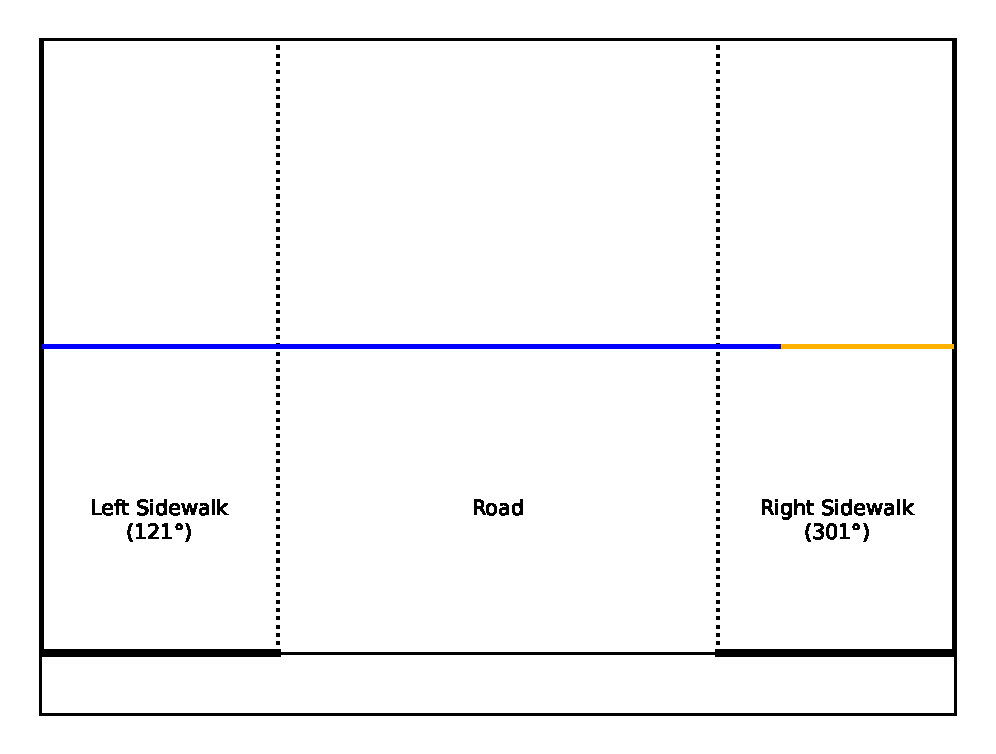
\includegraphics[width=\columnwidth]{sidewalk_predictions/shade_at_8}}
\end{center}
\caption{Street Scene with Shade for 8AM}
\label{prediction8}
\vskip -0.2in
\end{figure}

\section{Discussion}
\label{discussion}
This study has demonstrated the feasibility and effectiveness of a sophisticated digital tool for mapping shade scenarios in urban environments. An automated, user-friendly tool like this could revolutionize urban planning by enabling more efficient allocation of resources for shade improvement, ultimately leading to greater pedestrian well-being.

Despite achieving high accuracy rates of 81\% for the GSV to Sun Model and 92\% for our Sidewalk-Shifting model, there are areas where the work can be expanded and limitations that need to be addressed in future research. Our model for sidewalk shifting still heavily relies on the heights of the buildings near the image, which we did not have time to predict solely from the GSV data. Few works like \citet{YAN202283} exist in this field, and we believe integrating our solution with a model that predicts building heights could be highly beneficial.

Currently, our model requires the road angle as an input. To scale this system for larger areas without requiring individual input for each location, we could utilize available map data to determine road angles.

Similarly, understanding the heights of surrounding buildings is essential for improving our shade prediction. Rather than manually inputting this data, a more scalable approach would be integrating our model with city height maps. By integrating with such resources, our model can automatically acquire building heights, enabling the tool to be used across large urban areas without intensive data entry.

Once we have the heights of numerous surrounding buildings we could calculate the shade relative to the specific building that is covering the sun at that specific time.
\section{Code}
\label{code}
All of our code is available in - TODO - Link to clean Github (no commits)
Furthermore, our end to end solution was implemented on TAU Innovation Labs' servers, and we created a walkthrough and worked together with our colleagues to allow for their independent use of the system.

\section{Related Work}
\label{related-work}
Prior to commencing our project, we extensively reviewed various published articles that endeavored to address the identical challenge of harnessing Google Street View (GSV) for the purpose of predicting shading patterns. Notable contributions in this domain include \citet{DENG2021103289} and \citet{GONG2019547}.

In the context of our project, we drew inspiration from these existing works and amalgamated select components of their methodologies, particularly in the segment related to fisheye image processing and overall pipeline flow. We adapted and integrated certain elements from these articles.

In our project we have enhanced the pipeline by refining segmentation and classification techniques, and have successfully integrated an initial Proof of Concept to evaluate sidewalk shading status.

\section{Acknowledgements}
\label{acknowledgements}
We would like to extend our gratitude to Iftah Giloh for his indispensable support and guidance throughout the course of this project.. We would also like to thank Dr. Amit Bermano, for his guidance on deep learning vision techniques that we considered using in this project.

\bibliography{final_paper}
\bibliographystyle{icml2022}

%%%%%%%%%%%%%%%%%%%%%%%%%%%%%%%%%%%%%%%%%%%%%%%%%%%%%%%%%%%%%%%%%%%%%%%%%%%%%%%
%%%%%%%%%%%%%%%%%%%%%%%%%%%%%%%%%%%%%%%%%%%%%%%%%%%%%%%%%%%%%%%%%%%%%%%%%%%%%%%
% APPENDIX
%%%%%%%%%%%%%%%%%%%%%%%%%%%%%%%%%%%%%%%%%%%%%%%%%%%%%%%%%%%%%%%%%%%%%%%%%%%%%%%
%%%%%%%%%%%%%%%%%%%%%%%%%%%%%%%%%%%%%%%%%%%%%%%%%%%%%%%%%%%%%%%%%%%%%%%%%%%%%%%
\newpage
\appendix
\section{Sidewalk Predictions}
\label{sidewalk-predictions}
Below are the predictions, as mentioned in Section \ref{sidewalk-shifting-results}.

\begin{figure}[ht]
\begin{center}
\centerline{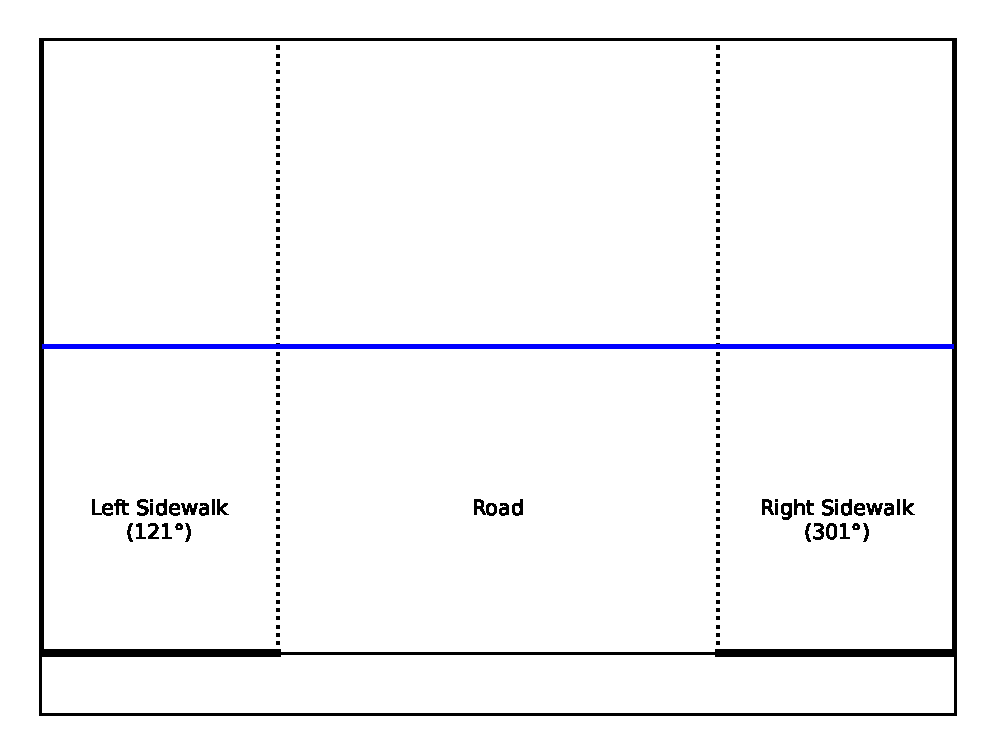
\includegraphics[width=\columnwidth]{sidewalk_predictions/shade_at_6}}
\caption{Street Scene with Shade for 6AM}
\end{center}
\end{figure}

\begin{figure}[ht]
\begin{center}
\centerline{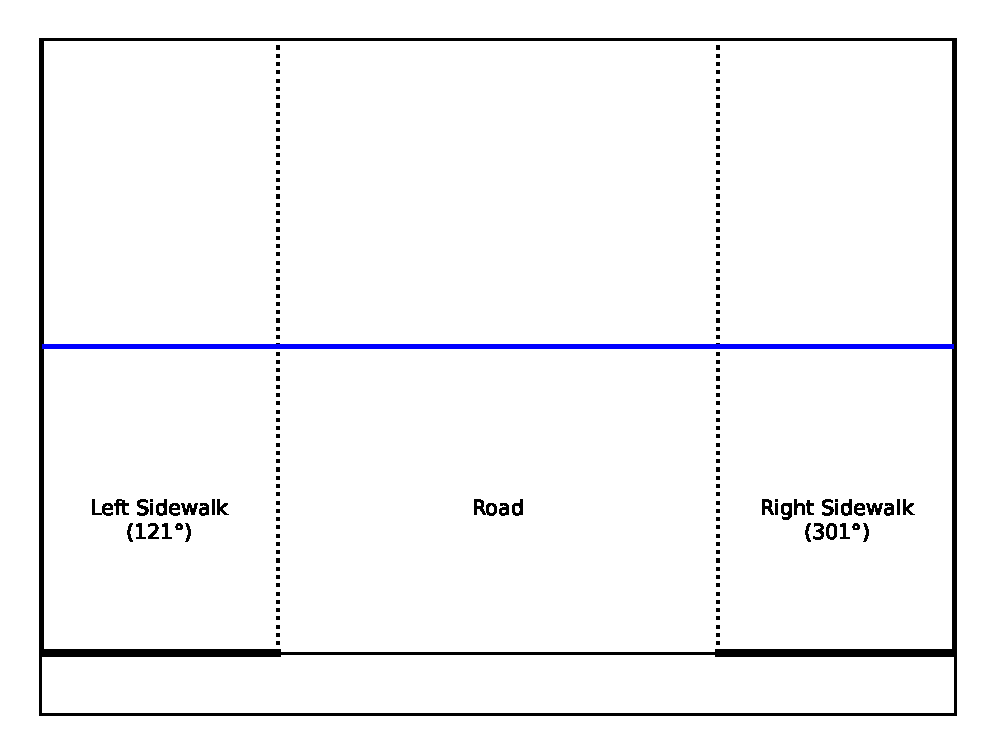
\includegraphics[width=\columnwidth]{sidewalk_predictions/shade_at_7}}
\caption{Street Scene with Shade for 7AM}
\end{center}
\end{figure}

\begin{figure}[ht]
\begin{center}
\centerline{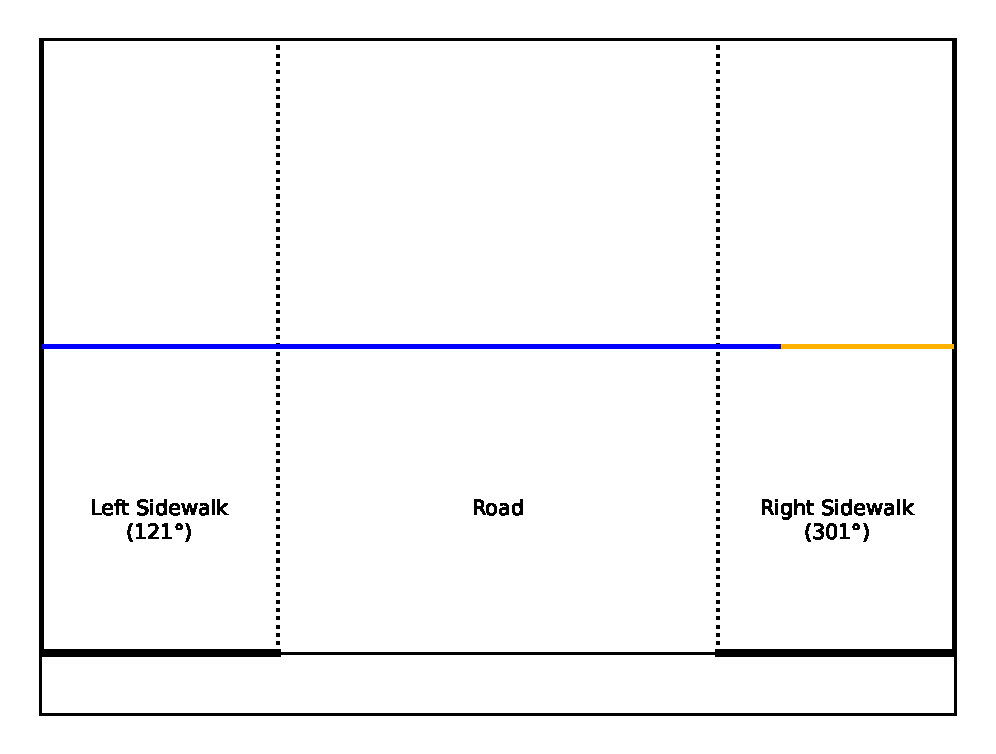
\includegraphics[width=\columnwidth]{sidewalk_predictions/shade_at_8}}
\caption{Street Scene with Shade for 8AM}
\end{center}
\end{figure}

\begin{figure}[ht]
\begin{center}
\centerline{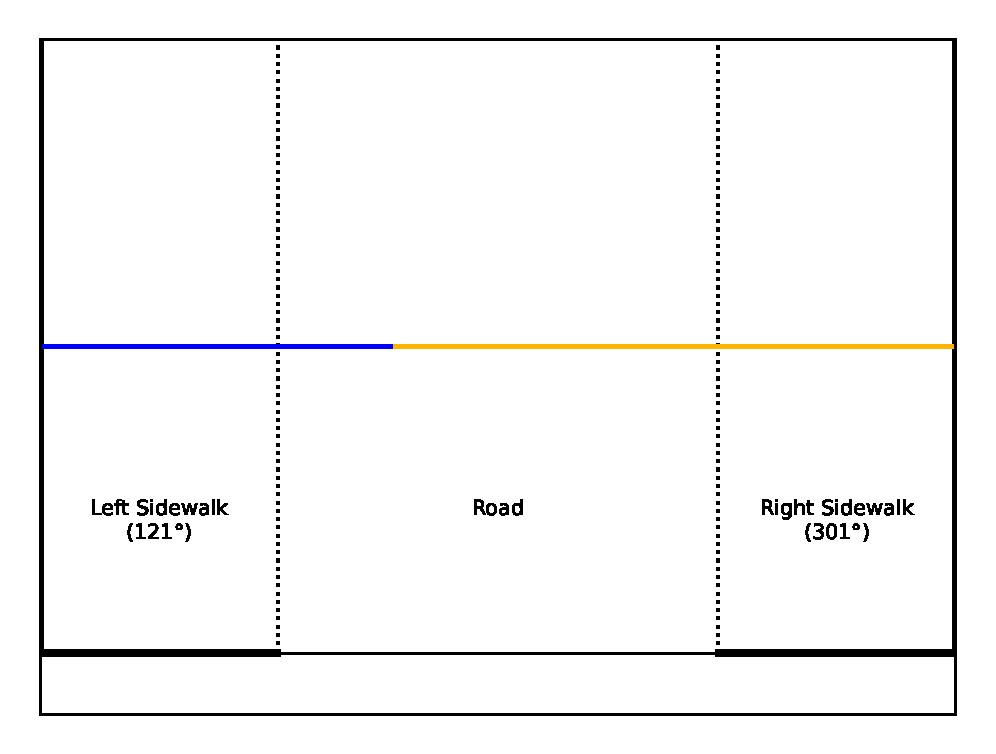
\includegraphics[width=\columnwidth]{sidewalk_predictions/shade_at_9}}
\caption{Street Scene with Shade for 9AM}
\end{center}
\end{figure}

\begin{figure}[ht]
\begin{center}
\centerline{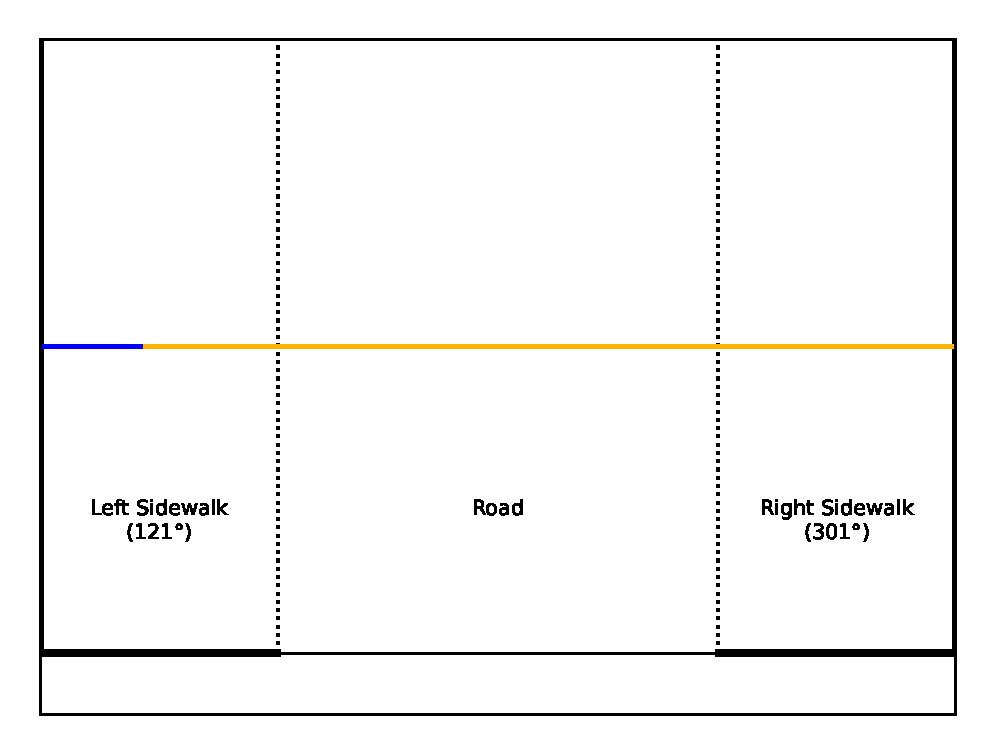
\includegraphics[width=\columnwidth]{sidewalk_predictions/shade_at_10}}
\caption{Street Scene with Shade for 10AM}
\end{center}
\end{figure}

\begin{figure}[ht]
\begin{center}
\centerline{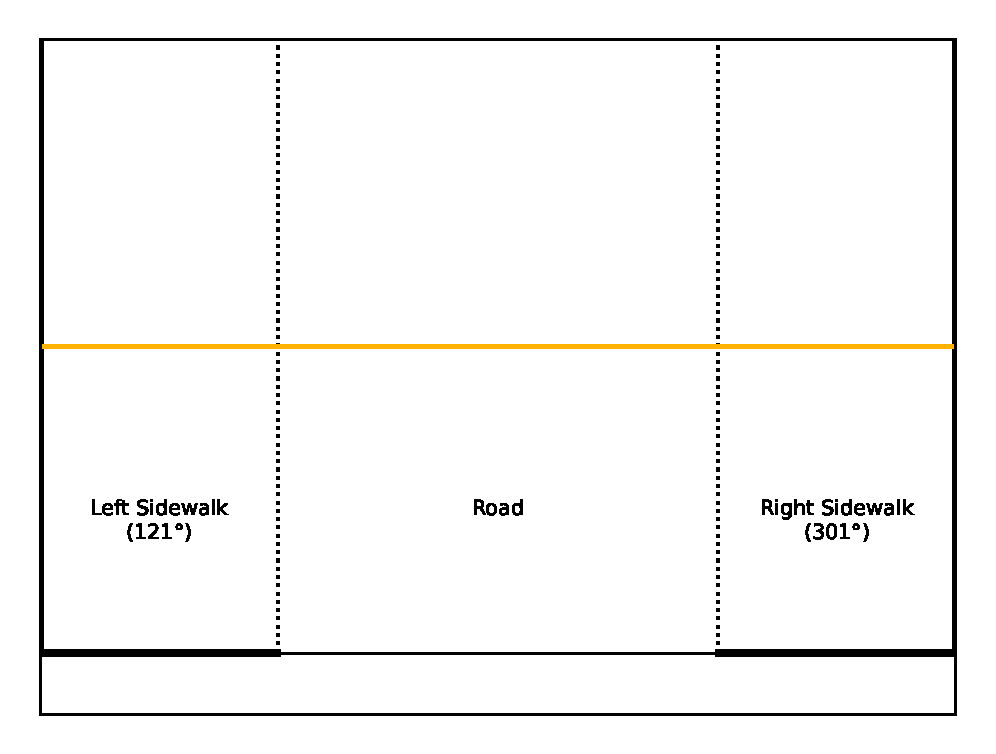
\includegraphics[width=\columnwidth]{sidewalk_predictions/shade_at_11}}
\caption{Street Scene with Shade for 11AM}
\end{center}
\end{figure}

\begin{figure}[ht]
\begin{center}
\centerline{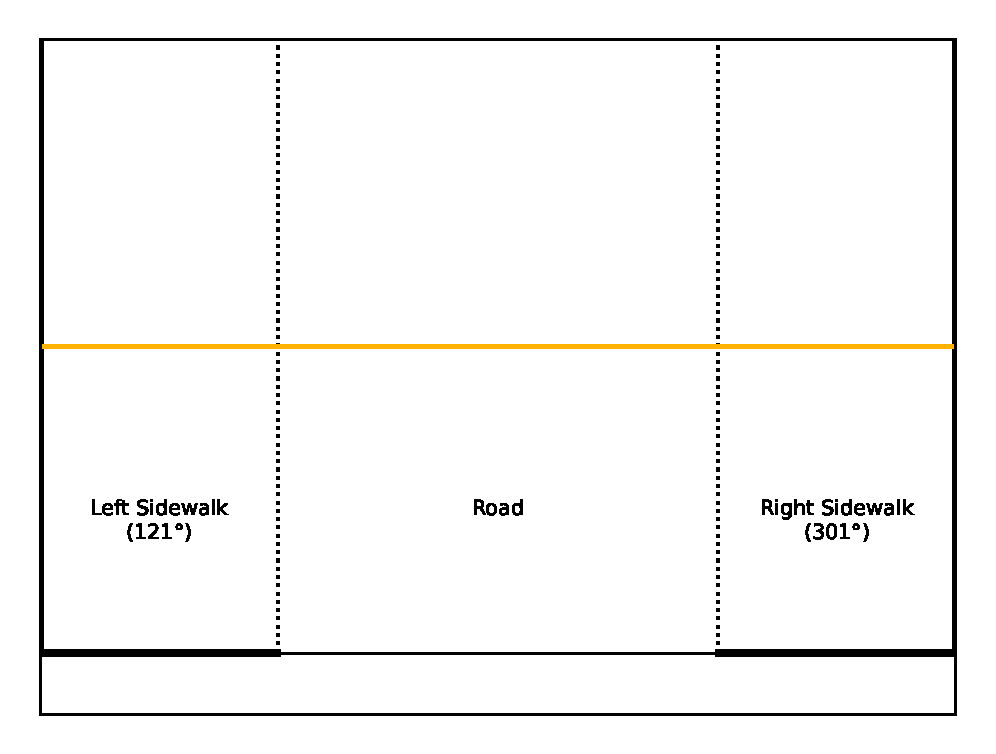
\includegraphics[width=\columnwidth]{sidewalk_predictions/shade_at_12}}
\caption{Street Scene with Shade for 12PM}
\end{center}
\end{figure}

\begin{figure}[ht]
\begin{center}
\centerline{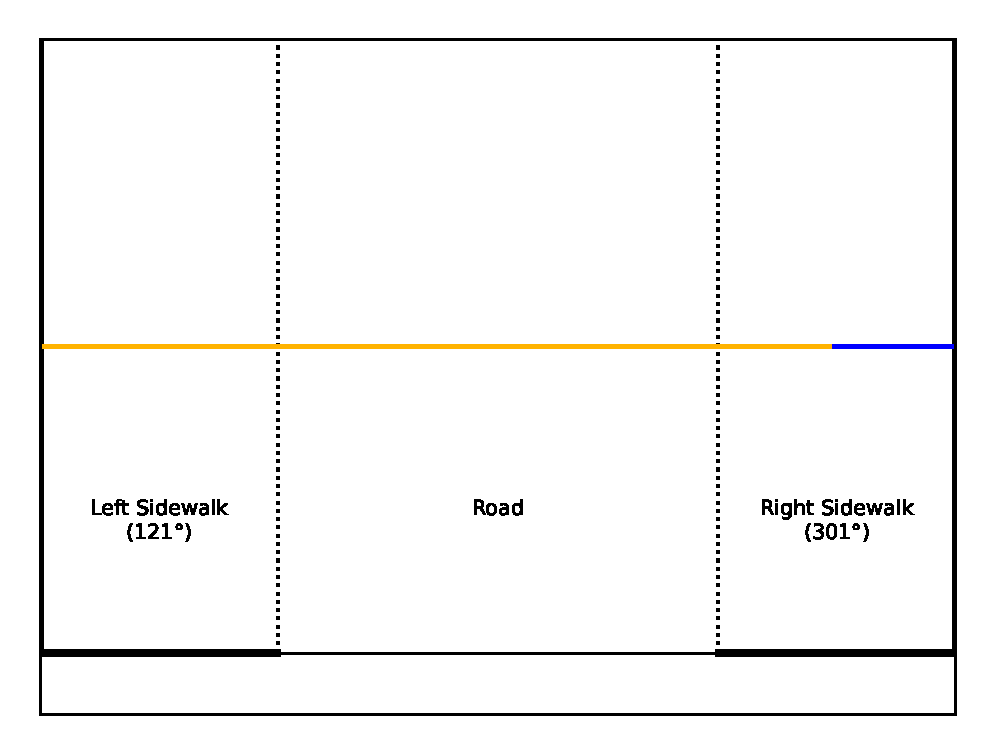
\includegraphics[width=\columnwidth]{sidewalk_predictions/shade_at_13}}
\caption{Street Scene with Shade for 13PM}
\end{center}
\end{figure}

\begin{figure}[ht]
\begin{center}
\centerline{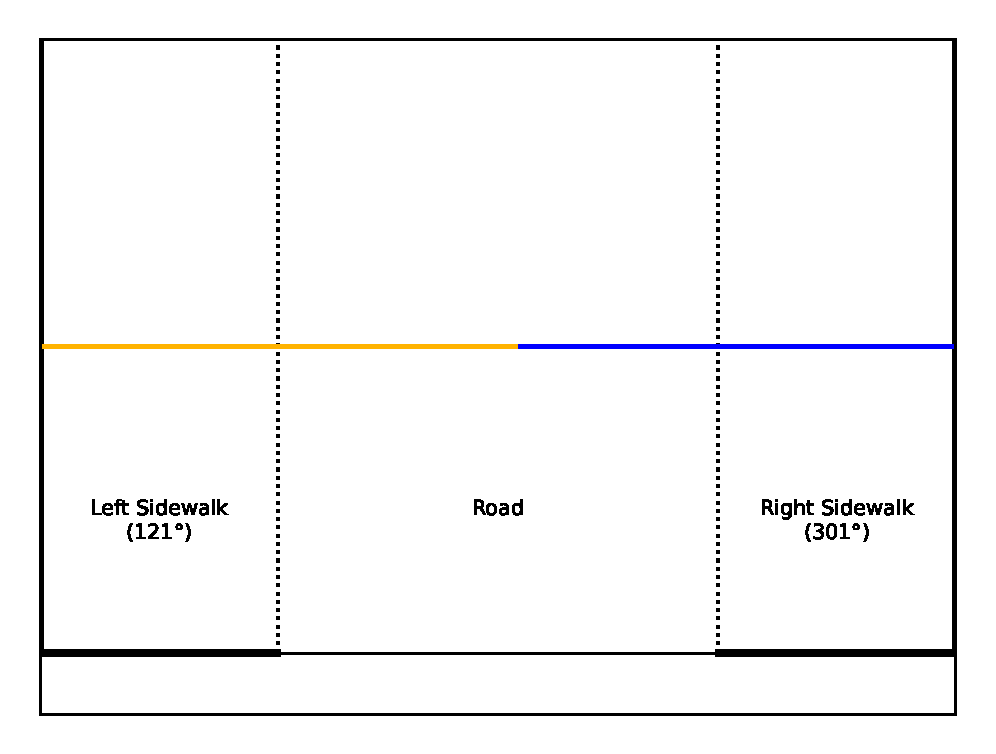
\includegraphics[width=\columnwidth]{sidewalk_predictions/shade_at_14}}
\caption{Street Scene with Shade for 14PM}
\end{center}
\end{figure}

\begin{figure}[ht]
\begin{center}
\centerline{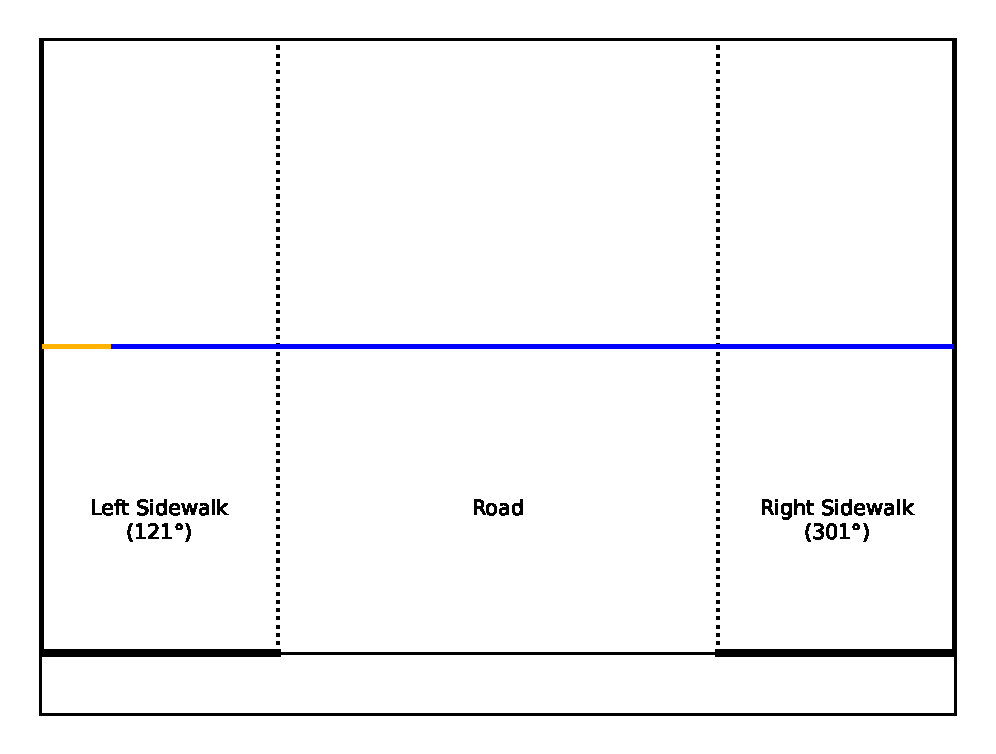
\includegraphics[width=\columnwidth]{sidewalk_predictions/shade_at_15}}
\caption{Street Scene with Shade for 15PM}
\end{center}
\end{figure}

\begin{figure}[ht]
\begin{center}
\centerline{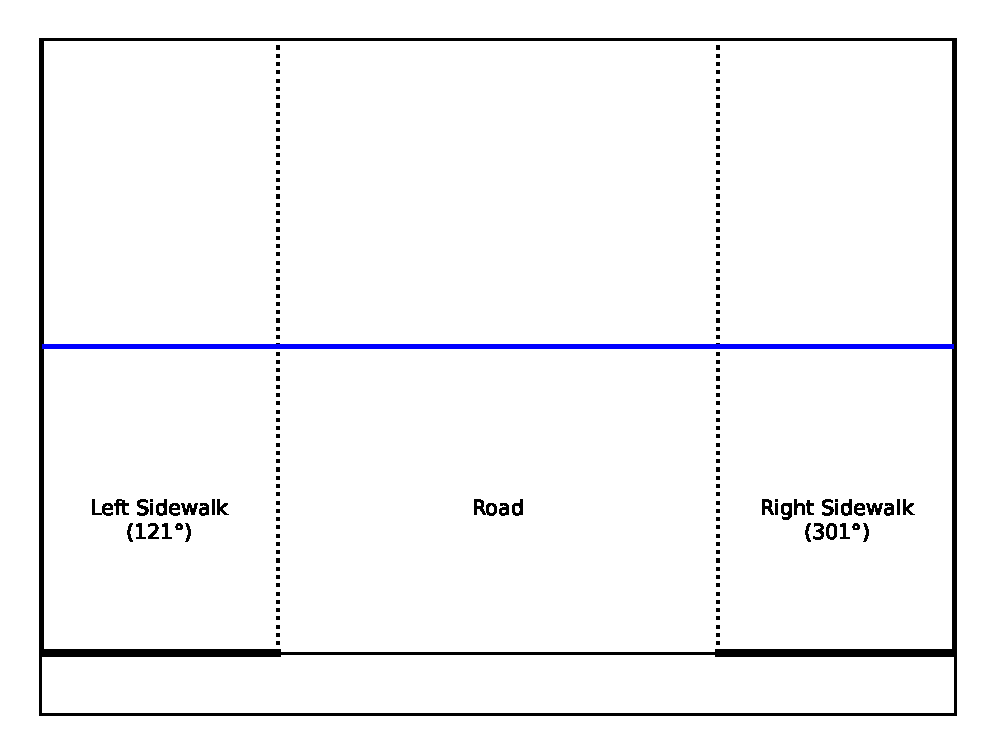
\includegraphics[width=\columnwidth]{sidewalk_predictions/shade_at_16}}
\caption{Street Scene with Shade for 16PM}
\end{center}
\end{figure}

\begin{figure}[ht]
\begin{center}
\centerline{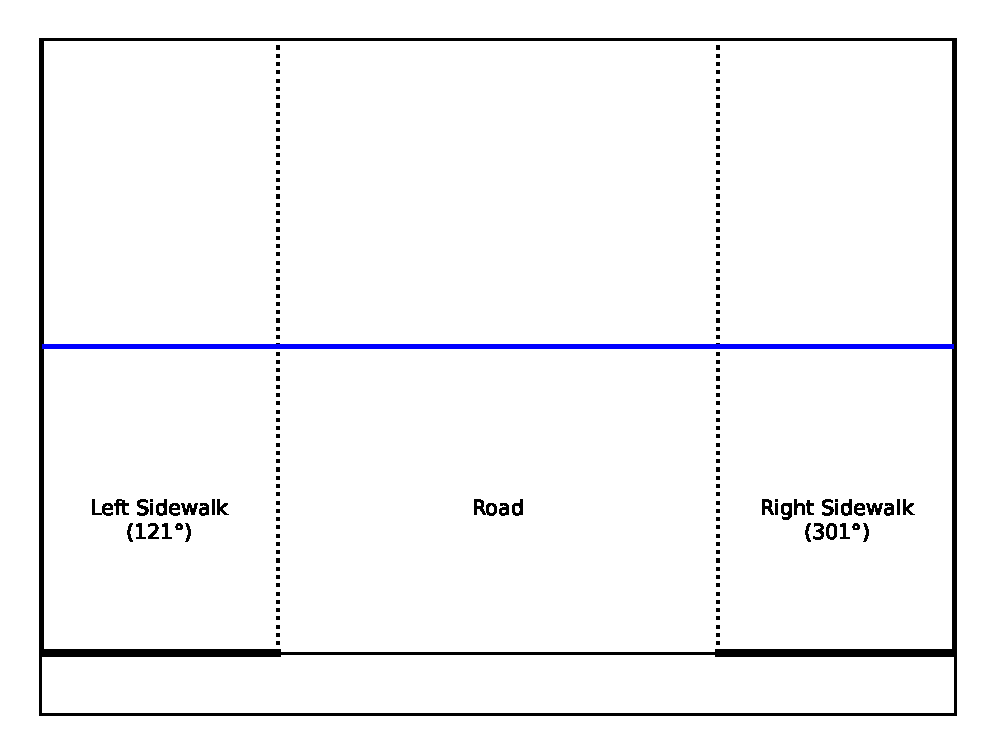
\includegraphics[width=\columnwidth]{sidewalk_predictions/shade_at_17}}
\caption{Street Scene with Shade for 17PM}
\end{center}
\end{figure}

\begin{figure}[ht]
\begin{center}
\centerline{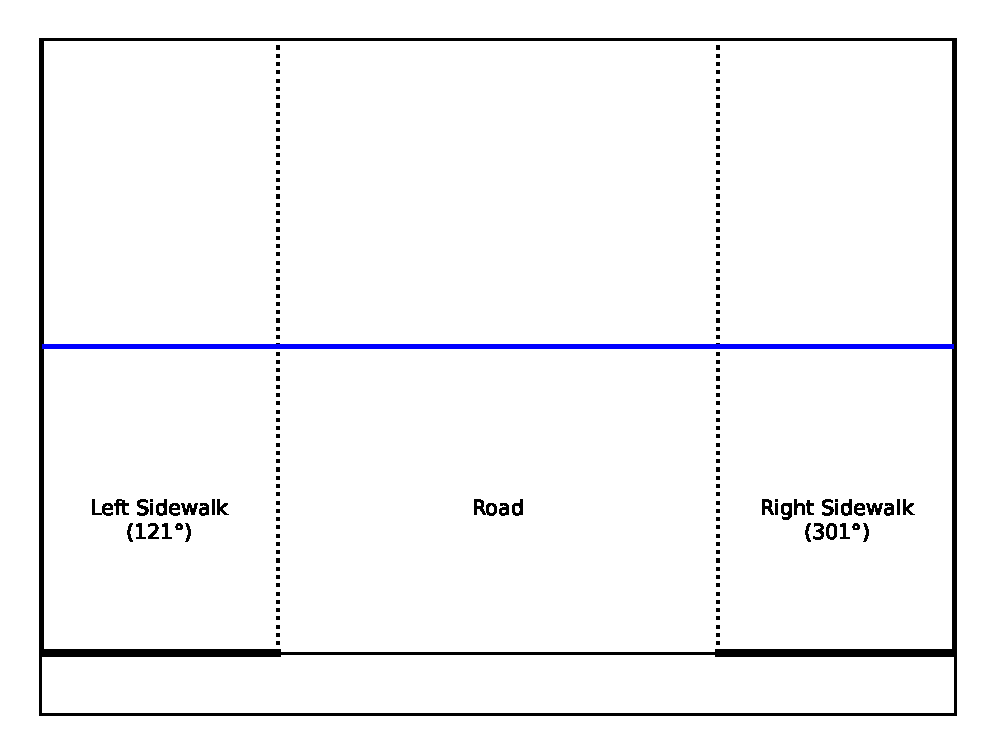
\includegraphics[width=\columnwidth]{sidewalk_predictions/shade_at_18}}
\caption{Street Scene with Shade for 18PM}
\end{center}
\end{figure}

\begin{figure}[ht]
\begin{center}
\centerline{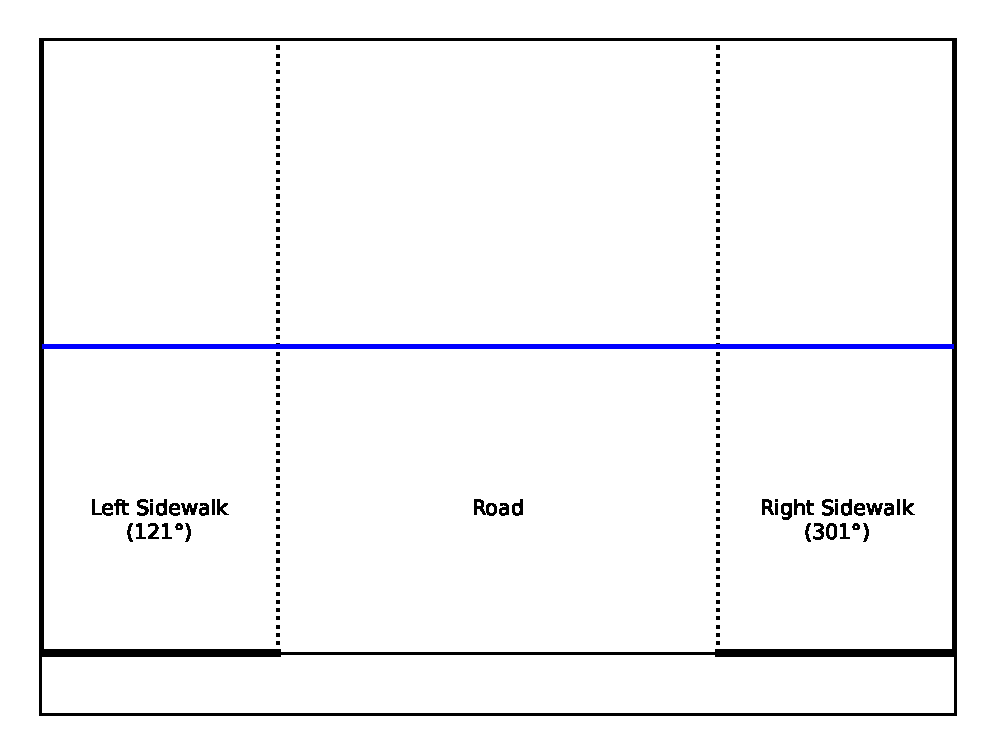
\includegraphics[width=\columnwidth]{sidewalk_predictions/shade_at_19}}
\caption{Street Scene with Shade for 19PM}
\end{center}
\end{figure}

%%%%%%%%%%%%%%%%%%%%%%%%%%%%%%%%%%%%%%%%%%%%%%%%%%%%%%%%%%%%%%%%%%%%%%%%%%%%%%%
%%%%%%%%%%%%%%%%%%%%%%%%%%%%%%%%%%%%%%%%%%%%%%%%%%%%%%%%%%%%%%%%%%%%%%%%%%%%%%%

\end{document}